\chapter{Unit Circle} \label{ch:unit-circle}

\section{Introduction}

The unit circle (Figure \ref{fig:unit-circle}) is a treasure trove of strange connections with other areas of mathematics, many of which are constantly useful in physics.

\begin{figure}[h]
    \centering
    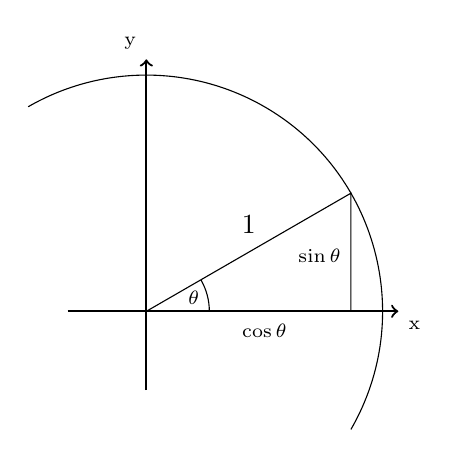
\begin{tikzpicture}
        \draw[thick,->] (-1,0) -- (3.2,0) node[anchor=north west] {\scriptsize x};
        \draw[thick,->] (0,-1) -- (0,3.2) node[anchor=south east] {\scriptsize y};
        \draw (2.598,-1.5) arc (-30:120:3);       
        \draw (0,0) -- (2.598,0) -- (2.598,1.5) -- cycle;
        \node at (1.5,-0.25) {\scriptsize $\cos \theta$};
        \node at (2.2,0.7) {\scriptsize $\sin \theta$};
        \node at (1.3,1.1) {$1$};
        \node at (0.6,0.17) {\scriptsize $\theta$};
        \draw (0.8,0) arc(0:30:0.8);
    \end{tikzpicture}
    \caption{The unit circle} \label{fig:unit-circle}
\end{figure}

The points that make up the circumference (edge) of a unit circle are all the points that are $1$ unit of distance from the centre. The same definition is used for a sphere in any number of spatial dimensions.

For historical reasons\footnote{The ratio between the diameter, $d$ of a circle and the circumference is $\pi$. But it has turned out over succeeding millennia that the radius $r = d/2$ is far more commonly encountered in calculations, and so we are doomed to say $2\pi$ almost everywhere.} when measuring distances travelled around the circumference of a unit circle we define the number $\pi$ to be the length of half a circumference, so length of the circumference of a unit circle is $2\pi$. We call this distance travelled around a part of the unit circle's circumference the \textit{angle}. By convention we always begin measuring the angle from the $x$-axis and moving in the counter-clockwise direction. In the figure the angle $\theta$ happens to be $\pi/6$, the same as 30$^\circ$.

\section{Sine and Cosine}

Given an angle, it is surely possible to compute the $(x, y)$ coordinates of the corresponding point on the circumference. There must exist a pair of functions that give these coordinates, traditionally named as follows:

\begin{itemize}
    \item $\sin \theta$ ("sine") gives the vertical or $y$ coordinate, and
    \item $\cos \theta$ ("cosine") gives the horizontal or $x$ coordinate.
\end{itemize}

Without knowing anything else about these functions, we can already see that as an object progresses around the circle, its coordinates must visit these milestones:

\begin{itemize}
    \item We begin at $\theta = 0$, the right-most point of the circle, where $\sin \theta = 0$ and $\cos \theta = 1$.
    \item At $\theta = \pi/2$ (90$^\circ$), the top of the circle, the situation has reversed: $\sin \theta = 1$ and $\cos \theta = 0$.
    \item At $\theta = \pi$ (180$^\circ$), the left-most point of the circle, $\sin \theta = 0$ and $\cos \theta = -1$.
    \item At $\theta = 3\pi/2$ (270$^\circ$), the bottom of the circle, $\sin \theta = -1$ and $\cos \theta = 0$.
\end{itemize}

We can plot $\sin \theta$ by itself (Figure \ref{fig:sin}) between the values $0$ and $2\pi$, and likewise $\cos \theta$ (Figure \ref{fig:cos}).

\begin{figure}[h]
    \caption{Sine and Cosine}
    \begin{subfigure}{0.5\textwidth}
        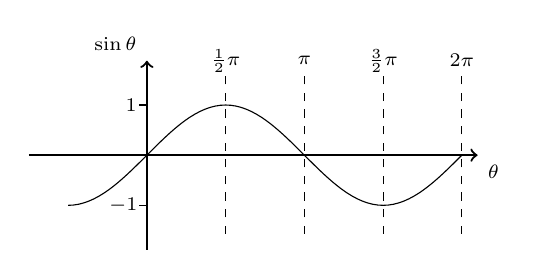
\begin{tikzpicture}
            \draw[thick,->] (-0.5,0) -- (5.2,0) node[anchor=north west] {\scriptsize $\theta$};
            \draw[thick,->] (1,-1.2) -- (1,1.2) node[anchor=south east] {\scriptsize $\sin \theta$};
            \draw (0,-0.637) cos(1,0) sin (2,0.637) cos (3,0) sin (4,-0.637) cos (5,0);
            \draw[dashed] (2,-1) -- (2,1);
            \draw[dashed] (3,-1) -- (3,1);
            \draw[dashed] (4,-1) -- (4,1);
            \draw[dashed] (5,-1) -- (5,1);
            \node at (2,1.2) {\scriptsize $\frac{1}{2}\pi$};            
            \node at (3,1.2) {\scriptsize $\pi$};            
            \node at (4,1.2) {\scriptsize $\frac{3}{2}\pi$};
            \node at (5,1.2) {\scriptsize $2\pi$};
            \draw (0.9,0.637) -- (1,0.637);
            \node at (0.8,0.637) {\scriptsize $1$};
            \draw (0.9,-0.637) -- (1,-0.637);
            \node at (0.7,-0.637) {\scriptsize $-1$};
        \end{tikzpicture}
    \caption{The $\sin$ function} \label{fig:sin}
    \end{subfigure}
    \begin{subfigure}{0.5\textwidth}
        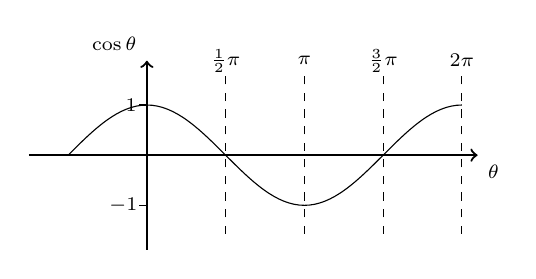
\begin{tikzpicture}
            \draw[thick,->] (-0.5,0) -- (5.2,0) node[anchor=north west] {\scriptsize $\theta$};
            \draw[thick,->] (1,-1.2) -- (1,1.2) node[anchor=south east] {\scriptsize $\cos \theta$};
            \draw (0,0) sin (1,0.637) cos (2,0) sin (3,-0.637) cos (4,0) sin(5, 0.637);
            \draw[dashed] (2,-1) -- (2,1);
            \draw[dashed] (3,-1) -- (3,1);
            \draw[dashed] (4,-1) -- (4,1);
            \draw[dashed] (5,-1) -- (5,1);
            \node at (2,1.2) {\scriptsize $\frac{1}{2}\pi$};            
            \node at (3,1.2) {\scriptsize $\pi$};            
            \node at (4,1.2) {\scriptsize $\frac{3}{2}\pi$};
            \node at (5,1.2) {\scriptsize $2\pi$};
            \draw (0.9,0.637) -- (1,0.637);
            \node at (0.8,0.637) {\scriptsize $1$};
            \draw (0.9,-0.637) -- (1,-0.637);
            \node at (0.7,-0.637) {\scriptsize $-1$};
        \end{tikzpicture}
        \caption{The $\cos$ function} \label{fig:cos}
    \end{subfigure}
\end{figure}

We can see that $\cos$ is just $\sin$ advanced by a quarter of a cycle, or:

$$
\cos \theta = \sin (\theta + \pi/2)
$$ 

If we advanced $\sin$ by $\pi$, half a cycle, the peaks and valleys would change places, while the uphill slopes that cut through the horizontal axis would become downhill slopes and vice versa. In other words, it would look exactly like we'd flipped the $\sin$ function upside down:

\begin{figure}[h]
    \centering
    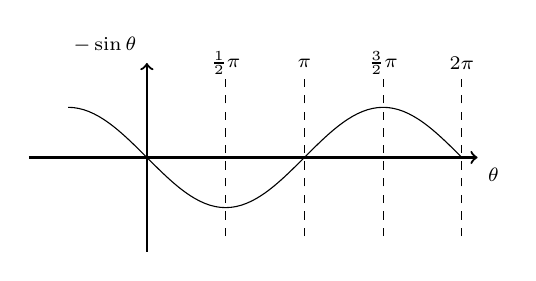
\begin{tikzpicture}
        \draw[thick,->] (-0.5,0) -- (5.2,0) node[anchor=north west] {\scriptsize $\theta$};
        \draw[thick,->] (1,-1.2) -- (1,1.2) node[anchor=south east] {\scriptsize $-\sin \theta$};
        \draw (0,0.637) cos(1,0) sin (2,-0.637) cos (3,0) sin (4,0.637) cos (5,0);
        \draw[dashed] (2,-1) -- (2,1);
        \draw[dashed] (3,-1) -- (3,1);
        \draw[dashed] (4,-1) -- (4,1);
        \draw[dashed] (5,-1) -- (5,1);
        \node at (2,1.2) {\scriptsize $\frac{1}{2}\pi$};            
        \node at (3,1.2) {\scriptsize $\pi$};            
        \node at (4,1.2) {\scriptsize $\frac{3}{2}\pi$};
        \node at (5,1.2) {\scriptsize $2\pi$};        
    \end{tikzpicture}
    \caption{$\sin \theta$ upside down} \label{fig:minus-sin}
\end{figure}

So:

$$
-\sin \theta = \cos (\theta + \pi/2) = \sin (\theta + \pi)
$$

Incidentally, the word \textit{cycle} is from the Greek word for circle. The word \textit{phase} is also used a lot in this context, probably deriving from the phases of the moon. When one periodic function is equal to another shifted by some amount, we say there is only a phase difference between them.

\section{Differential Calculus on Sine and Cosine}

Think of an object moving along the unit circle's edge at a constant rate. It has an instantaneous velocity vector pointing along the tangent, but this is always at a right angle to the line segment reaching from the centre to the object (the radius).

\begin{figure}[h]
    \centering
    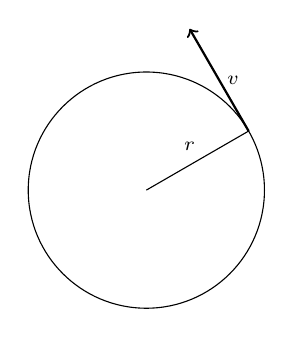
\begin{tikzpicture}
        \draw (0,0) circle(1.5);
        \draw (0,0) -- (1.299,0.75);
        \draw[thick,->] (1.299,0.75) -- (0.549,2.049);
        \node at (0.55,0.55) {\scriptsize $r$};
        \node at (1.1,1.4) {\scriptsize $v$};
            
    \end{tikzpicture}
    \caption{The velocity vector $v$ of an orbiting object} \label{fig:circle-tangent}
\end{figure}

The velocity vector is therefore fixed to be a quarter cycle ahead of the radius, which is precisely the relationship between $\cos \theta$ and $\sin \theta$. The components of $v$ are the rates at which the corresponding components of $r$ change as the angle advances. It follows that the rate at which $\sin \theta$ is increasing is given by $\cos \theta$, or:

$$
\frac{d}{d\theta} \sin \theta = \cos \theta
$$

This is confirmed by examining the shape of the functions separately. Nearby to $\theta = 0$, $\sin \theta$ is closely approximated by $\theta$ itself, and looks (Figure \ref{fig:sin-small}) much like a straight line of gradient $1$, which happens to be the value of $\cos 0$.

\begin{figure}[h]    
    \caption{Gradients of Sine}
    \begin{subfigure}{0.5\textwidth}
        \centering
        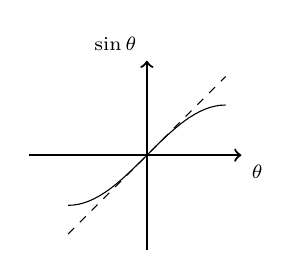
\begin{tikzpicture}
            \draw[thick,->] (-0.5,0) -- (2.2,0) node[anchor=north west] {\scriptsize $\theta$};
            \draw[thick,->] (1,-1.2) -- (1,1.2) node[anchor=south east] {\scriptsize $\sin \theta$};
            \draw (0,-0.637) cos(1,0) sin (2,0.637);
            \draw[dashed] (0,-1) -- (2,1);
        \end{tikzpicture}
    \caption{$\sin \theta \approx \theta$} \label{fig:sin-small}
    \end{subfigure}
    \begin{subfigure}{0.5\textwidth}
        \centering
        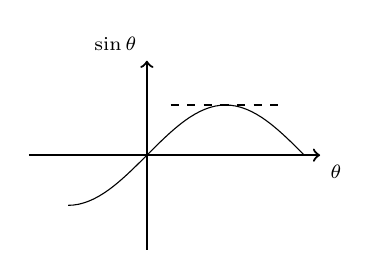
\begin{tikzpicture}
            \draw[thick,->] (-0.5,0) -- (3.2,0) node[anchor=north west] {\scriptsize $\theta$};
            \draw[thick,->] (1,-1.2) -- (1,1.2) node[anchor=south east] {\scriptsize $\sin \theta$};
            \draw (0,-0.637) cos(1,0) sin (2,0.637) cos (3,0);
            \draw[dashed] (1.3,0.637) -- (2.7,0.637);
        \end{tikzpicture}
        \caption{Gradient $0$} \label{fig:sin-peak}
    \end{subfigure}
\end{figure}

When $\sin \theta$ peaks at $\theta = \pi/2$, its gradient is $0$, and again this is in agreement with the value of $\cos (\pi/2)$. This pattern continues at every point in the cycle.

So in any situation where we need the derivative of $\sin$, we just replace it with $\cos$. By the same reasoning (and because we know the same relationship exists between $-\sin \theta$ and $\cos \theta$) we can assume that:
$$
\frac{d}{d\theta} \cos \theta = -\sin \theta
$$

Differentiating two more times will get us back to $\sin \theta$ because each differentiation advances the function by a quarter cycle. Naturally integration performs the same trick in the opposite direction.

\section{Computing Sine and Cosine} \label{sec:unit-circle-maclaurin}

Now we can take the derivative of $\sin$, and we know its precise value at $0$ (and those of its derivatives), we can use the Maclaurin method to find how to compute it using only addition and multiplication, if only we have the patience to perform an infinite sequence of those operations. We begin by assuming that a function $f(x)$ can be expressed as the sum of an infinite series of polynomial terms, that is, some constant $a_n$ multiplied by the variable $x$ raised to an integer power $n$, beginning at $0$:

$$
f(x) = a_0x^0 + a_1x^1 + a_2x^2 + a_3x^3 + \ldots
$$

Anything raised to the power of $0$ is $1$, and raising something to the power of $1$ makes no difference, so at the expense of consistency, and meanwhile also naming the function we want to compute, we just write:

$$
\sin x = a_0 + a_1x + a_2x^2 + a_3x^3 + \ldots
$$

So we only need to determine the constant factors $a_n$ to entirely characterise the function. Setting $x = 0$, any term that is multiplied by $x$ must be zero (they \textit{vanish} entirely from the sum), which only leaves $a_0$. But $\sin 0 = 0$, so it follows that $a_0 = 0$. Taking the derivative of both sides:

$$
\cos x = a_1 + 2a_2x + 3a_3x^2 + 4a_4x^3 + \ldots
$$

Each polynomial's power is reduced by $1$, and the original power "moves down" to become an extra factor. Now the exact same vanishing argument applies to $a_1$ except that here it is solely responsible for the value of $\cos 0 = 1$, and so it must be that $a_1 = 1$. We differentiate a second time:

$$
-\sin x = 2a_2 + (3\cdot2)a_3x + (4\cdot3)a_4x^2 + \ldots
$$

So $a_2 = 0$. Differentiate a third time:

$$
-\cos x = (3\cdot2)a_3 + (4\cdot3\cdot2)a_4x + \ldots
$$

So $a_3 = -\frac{1}{3!}$. When $n$ is even the term is zero, and when $n$ is odd the term $x^n$ is divided by the accumulated value $n!$. We continue in this fashion to find that:

$$
\sin x = x - \frac{x^3}{3!} + \frac{x^5}{5!} - \frac{x^7}{7!} + \frac{x^9}{9!} - \ldots
$$

By the same process we find that for $cos$ only the even-$n$ terms appear in the result:

$$
\cos x = 1 - \frac{x^2}{2!} + \frac{x^4}{4!} - \frac{x^6}{6!} + \frac{x^8}{8!} - \ldots
$$

In each case there is a four stage cycle, with alternating absence of terms and then similarly alternating $+$/$-$ signs. This is curiously reminiscent of the cyclic behaviour of imaginary unit number $i$, defined such that $i^2 = -1$, as we raise it to integer powers starting at zero:

\begin{itemize}
    \item $i^0 = 1$
    \item $i^1 = i$
    \item $i^2 = -1$
    \item $i^3 = i(i^2) = -i$
    \item $i^4 = (i^2)(i^2) = (-1)(-1) = 1$
    \item and so on: $i$, $-1$, $-i$, $1$, $i$, $-1$ $\ldots$
\end{itemize}

\section{Euler's Formula} \label{euler-formula}

If we get carried away by the power of this method we risk drifting from the topic of the unit circle, but it turns out that there is no escape.

The exponential function $e^x$ raises the constant $e$ to a variable power, and the value $e$ is chosen such that the derivative is $e^x$, so the function is its own derivative. The method of evaluating at zero and taking repeated derivatives is therefore particularly simple to perform and yields:

$$
e^x = 1 + x + \frac{x^2}{2!} + \frac{x^3}{3!} + \frac{x^4}{4!} + \frac{x^5}{5!} + \ldots
$$

This is obviously different from the previous two examples because no terms vanish and all terms are positive. But what happens if we replace $x$ with $xi$?

$$
e^{ix} = 1 + ix + \frac{i^2x^2}{2!} + \frac{i^3x^3}{3!} + \frac{i^4x^4}{4!} + \frac{i^5x^5}{5!} + \ldots
$$

Simplifying the various powers of $i$ according to its definition:

$$
e^{ix} = 1 + ix - \frac{x^2}{2!} - i\frac{x^3}{3!} + \frac{x^4}{4!} + i\frac{x^5}{5!} + \ldots
$$

It appears we can write it as the sum of two series, one containing only real terms and the other only imaginary:

$$
e^{ix} = (1 - \frac{x^2}{2!} + \frac{x^4}{4!} - \ldots) + i(x - \frac{x^3}{3!} + \frac{x^5}{5!} - \ldots)
$$

But the real component is evidently $\cos x$ while the imaginary one is $\sin x$!

$$
e^{ix} = \cos x + i\sin x
$$

This means that $x$ is the angle, so we will resuming calling it $\theta$. We can interpret $e^{i\theta}$ as a unit circle in the complex plane. It is all the complex numbers of modulus 1.

We can relabel the axes on our diagram of the unit circle, to show the circle in the complex plane (Figure \ref{fig:unit-circle-complex}).

\begin{figure}[h]
    \centering
    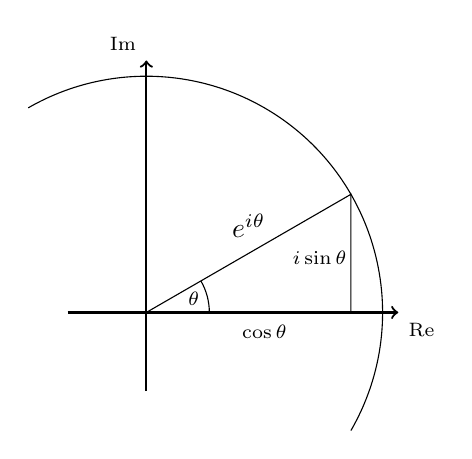
\begin{tikzpicture}
        \draw[thick,->] (-1,0) -- (3.2,0) node[anchor=north west] {\scriptsize Re};
        \draw[thick,->] (0,-1) -- (0,3.2) node[anchor=south east] {\scriptsize Im};
        \draw (2.598,-1.5) arc (-30:120:3);
        \draw (0,0) -- (2.598,0) -- (2.598,1.5) -- cycle;
        \node at (1.5,-0.25) {\scriptsize $\cos \theta$};
        \node at (2.2,0.7) {\scriptsize $i\sin \theta$};
        \node at (1.3,1.1) {$e^{i\theta}$};
        \node at (0.6,0.17) {\scriptsize $\theta$};
        \draw (0.8,0) arc(0:30:0.8);
    \end{tikzpicture}
    \caption{The unit circle in the complex plane} \label{fig:unit-circle-complex}
\end{figure}

We can scale the circle to any radius $r$ simply by multiplying by that radius. This means we can represent any complex number either as a sum $x + yi$, or as an exponential $re^{i\theta}$.

Physics is thick with examples of oscillation. To describe the state of a particle undergoing simple harmonic motion along a line, we need to know the position and the momentum. But a complex number, being described by two real numbers, can encapsulate both these quantities, and the real and imaginary parts have the right phase relationship.

\section{Pythagoras in the Circle}

There is a right-triangle in the diagram, so by Pythagoras:

$$
x^2 + y^2 = 1
$$

it must be that:

$$
(\sin \theta)^2 + (\cos \theta)^2 = 1
$$

Also by Pythagoras, given one coordinate of a point on the circle, we can compute the other:

\begin{center}
    $y = \sqrt{1 - x^2}$ \quad $x = \sqrt{1 - y^2}$    
\end{center}
